\documentclass[11pt]{article}

\usepackage{amsmath, amssymb, amsthm, mathtools}
\usepackage[margin=1in]{geometry}
\usepackage{booktabs, array, tabularx, longtable}
\usepackage{graphicx}
\usepackage{xcolor}
\usepackage{enumitem}
\usepackage{microtype}
\usepackage{algorithm}
\usepackage{algpseudocode}
\usepackage[colorlinks=true, linkcolor=blue!60!black, citecolor=blue!60!black, urlcolor=blue!60!black]{hyperref}
\setlength{\emergencystretch}{3em}

\theoremstyle{definition}
\newtheorem{definition}{Definition}
\newtheorem{remark}{Remark}
\newtheorem{obligation}{Obligation}
\theoremstyle{plain}
\newtheorem{theorem}{Theorem}
\newtheorem{lemma}{Lemma}
\newtheorem{proposition}{Proposition}

% ---------- macros ----------
\newcommand{\Rp}{\mathsf{R}}
\newcommand{\Op}{\mathsf{O}}
\newcommand{\Z}{\mathbb{Z}}
\newcommand{\Rq}{\mathcal{R}_q}
\newcommand{\Ecd}{\mathsf{Ecd}}
\newcommand{\Dcd}{\mathsf{Dcd}}
\newcommand{\Enc}{\mathsf{Enc}}
\newcommand{\bX}{\mathbf{X}}
\newcommand{\bA}{\mathbf{A}}
\newcommand{\bB}{\mathbf{B}}
\newcommand{\bC}{\mathbf{C}}
\newcommand{\bG}{\mathbf{G}}
\newcommand{\bI}{\mathbf{I}}
\newcommand{\bP}{\mathbf{P}}
\newcommand{\bV}{\mathbf{V}}
\newcommand{\bb}{\mathbf{b}}
\newcommand{\bc}{\mathbf{c}}
\newcommand{\by}{\mathbf{y}}
\newcommand{\bx}{\mathbf{x}}
\newcommand{\bxd}{\dot{\mathbf{x}}}
\newcommand{\btheta}{\boldsymbol{\theta}}
\newcommand{\bbeta}{\boldsymbol{\beta}}
\newcommand{\DG}{\mathcal{N}_{\Z}}
\newcommand{\PiO}{\Pi_O}
\DeclareMathOperator{\triu}{triu}
\DeclareMathOperator{\tr}{tr}
\algrenewcommand\algorithmicrequire{\textbf{Input:}}
\algrenewcommand\algorithmicensure{\textbf{Output:}}
\newcommand{\Rdo}{\textbf{\textcolor{blue!60!black}{R:}}\ }
\newcommand{\Odo}{\textbf{\textcolor{orange!70!black}{O:}}\ }
\newcommand{\Bdo}{\textbf{Both:}\ }

\title{\textbf{Protocol v3.1}\\[4pt]
\large Two-party vertical federated regression with threshold decryption\\ and lattice DP releases, under the honest-but-curious model}
\date{Draft for review}

\begin{document}
\maketitle

\begin{abstract}
\noindent
A researcher $\Rp$ holds a cohort with features $\bX_R$. An organization $\Op$ holds a register with features $\bX_O$ and the response $\by$. Protocol v3.1 computes a ridge-regularized least-squares fit over the records they share, together with confidence intervals. It reveals nothing to $\Op$ beyond public sizes, and it gives $\Rp$ only differentially private releases of the statistics that depend on $\Op$'s data.

v3.1 revises v3 to fix the four critical issues raised by the independent review of v3, under the honest-but-curious model. It also includes the review's other fixes that apply under this model. The key changes are four:
\begin{itemize}[nosep]
  \item $\Op$'s decryption share carries the DP noise, and the ciphertext component $c_0'$ is never transmitted. This closes a key-share leak.
  \item The homomorphic input checks are removed. They addressed only a malicious researcher, and one of them could be bypassed.
  \item Every error term that depends on $\Op$'s data or secrets is flooded statistically, in $\ell_2$, by the DP noise itself.
  \item The ridge is chosen from a separate first release, so it is independent of the noise in the release used for estimation.
\end{itemize}
Security against a deviating researcher is stated as an extension that requires zero-knowledge input proofs.
\end{abstract}

% ==============================================================
\section{Setting, threat model and guarantees}
\label{sec:model}

\paragraph{Data.} $\Op$ restricts its register to a study scope $D_\Phi=\{j:\Phi(j)\}$, where the predicate $\Phi$ uses public attributes only, such as province and birth-year band. $\Op$ pads $D_\Phi$ with dummy rows (fresh random identifiers that never match, with $\bx_O=\mathbf{0}$ and $y=0$) to a public size $\bar n_O$. $\Rp$ holds $n_R\le n_R^{\max}$ cohort records. Let $I$ be the cohort members that appear in $D_\Phi$, and $n=|I|$. The target is the ridge fit on $\bG=\bX^{I\top}\bX^{I}$ and $\bc=\bX^{I\top}\by^I$ over $\bX^I=[\bX_R^I\mid\bX_O^I]$, with $p=d_R+1+d_O$ columns, where the $+1$ is $\Rp$'s intercept. In block form,
\[
  \bG=\begin{pmatrix}\bA & \bC\\ \bC^\top & \bB\end{pmatrix},\qquad
  \bc=\begin{pmatrix}\bc_R\\ \bc_O\end{pmatrix},
\]
where $\bA=\bX_R^{I\top}\bX_R^{I}$ is $\Rp$'s own block, and $\bB,\bC,\bc_R,\bc_O,\by^\top\by$ depend on $\Op$'s data.

\paragraph{Preprocessing.} Before the protocol, each party transforms its own columns with constants agreed in Setup from public reference data or domain knowledge (\textsc{Preprocess}, Algorithm~\ref{alg:sub}): it standardizes each column; it may apply a per-column tail transform (winsorizing at $|z|\le c$, a rank-Gaussian transform from public reference quantiles, or a log transform); and it may normalize its own block of every row to unit norm ($\Rp$ without the intercept, so $\|\bxd\|^2=2$; $\Op$ gets $\|\bx_O\|=1$), optionally appending a clipped log of the block norm as a feature. $\Op$ treats $y$ the same way, except for block normalization. No transform uses the other party's columns, so no joint computation is needed. Each transform is a fixed function of one record and public constants, so one changed raw record changes one transformed record, and the adjacency and sensitivity analysis apply unchanged to the transformed data, with the bounds chosen on the transformed reference data. $\Op$'s constants must be data-independent, like \textsc{Calibrate}'s outputs; $\Rp$ may use its own constants, but it commits to $B_R$. Block normalization changes the meaning of the coefficients and is intended for prediction; winsorizing and log transforms keep them interpretable. Joint normalization of whole rows is not used: it would make $\bA$ depend on $\Op$'s data and need nonlinear functions under encryption, and on real data a joint norm budget gave little or no gain, because heavy tails, not the lack of a joint bound, make the bounds loose.

\paragraph{Threat model.} Both parties are \emph{honest-but-curious}. They follow the protocol, including key generation and $\Rp$'s preparation of its inputs (clipping, the selection vector), and they try to learn what they can from their views. Channels are private and authenticated. $\Rp$ is the analyst and receives the output.

\begin{definition}[Datasets and adjacency]
A dataset is $\Op$'s padded scope register $D=\{(\mathrm{id}_j,\bx_{O,j},y_j)\}_{j\le\bar n_O}$, with the cohort $(\mathrm{id},\bX_R)$, the identifiers and $\Phi$ held fixed. $D\sim D'$ if they differ in $(\bx_O,y)$ of exactly one row, matched or not.
\end{definition}

\begin{definition}[SIM-CDP and IND-CDP, after Mironov, Pandey, Reingold and Vadhan, 2009]
A protocol is $(\varepsilon,\delta)$-SIM-CDP for $\Rp$ with statistical slack $\gamma$ if there exist a mechanism $\mathcal{M}$ that is $(\varepsilon,\delta)$-DP with respect to $\sim$ and a probabilistic polynomial-time simulator $\mathcal{S}$ such that, for every $D$ and every PPT distinguisher $\mathcal A$, $|\Pr[\mathcal A(\mathrm{view}_{\Rp}(D))=1]-\Pr[\mathcal A(\mathcal{S}(\mathcal{M}(D)))=1]|\le\gamma+\mathrm{negl}(\lambda_{\mathrm{sec}})$. It is $(\varepsilon,\delta)$-IND-CDP if $\Pr[\mathcal A(\mathrm{view}_{\Rp}(D))=1]\le e^\varepsilon\Pr[\mathcal A(\mathrm{view}_{\Rp}(D'))=1]+\delta+\mathrm{negl}(\lambda_{\mathrm{sec}})$ for all $D\sim D'$. SIM-CDP with slack $\gamma$ implies IND-CDP with $\delta+(1+e^\varepsilon)\gamma$.
\end{definition}

\begin{table}[h]
\centering\small
\begin{tabularx}{\textwidth}{@{}l>{\raggedright\arraybackslash}X>{\raggedright\arraybackslash}X@{}}
\toprule
 & Guarantee & Basis \\
\midrule
G1 & \textbf{$\Rp$-input privacy}: $\Op$'s view can be simulated from $(n_R^{\max},\bar n_O)$ and the public parameters. & RLWE in $s_R$; security of the PSI. $\Op$ never receives a decryption share from $\Rp$. \\
G2 & \textbf{Cohort privacy}: $\Op$ learns nothing about $\Rp$'s cohort beyond $n_R^{\max}$. & Padded OPRF queries; labeled PSI (Chen et al., 2018). \\
G3 & \textbf{Output privacy}: per run, $(\varepsilon_{\mathrm{run}},\delta_{\mathrm{DP}})$-SIM-CDP with slack $\gamma$, hence $(\varepsilon_{\mathrm{run}},\delta_{\mathrm{run}})$-IND-CDP; over all runs on a base register, $(\varepsilon_L,\delta_L)$-IND-CDP. & Theorem~\ref{thm:output}; Proposition~\ref{prop:compose}. \\
G4 & \textbf{Disclosed}: $\Rp$ learns $I$ (which cohort members are in $D_\Phi$) and uniformly random positions $\tau(j)$, and nothing else about $\Op$'s register. & By design (Mode L; Remark~\ref{rem:modeM}); OPRF-keyed items and labels; \textsc{SanitizeBFV}. \\
\bottomrule
\end{tabularx}
\caption{Guarantees of v3.1 against honest-but-curious parties. Correctness assumes honest computation.}
\label{tab:guarantees}
\end{table}

% ==============================================================
\section{What changes relative to v3}
\label{sec:changes}

\begin{table}[h]
\centering\small
\begin{tabularx}{\textwidth}{@{}>{\raggedright\arraybackslash}p{4.3cm}>{\raggedright\arraybackslash}p{2.2cm}>{\raggedright\arraybackslash}X@{}}
\toprule
Critical issue in v3 & Exploitable by & Fix in v3.1 \\
\midrule
C1: $\Rp$ shifts its decryption share to pass the input check & malicious $\Rp$ & No homomorphic input check. Under the honest-but-curious model $\Rp$ prepares $\bb$ and $\dot\bX_R$ as specified (Algorithm~\ref{alg:upload}). The check, the slack vector and the relinearization and conjugation keys are all removed. Robustness to a deviating $\Rp$ is the extension in Section~\ref{sec:ext}. \\
C2: inputs that wrap around modulo $q$ pass the check & malicious $\Rp$ & As for C1. In addition, $q_0$ is sized so that honest inputs never wrap (Algorithm~\ref{alg:sub}, \textsc{Calibrate}). \\
C3: the release step leaks $\Op$'s key share & honest-but-curious $\Rp$ & $\Op$ sends $(c_1',h_O)$ with $h_O=c_0'+c_1's_O+\eta$; $c_0'$ is never transmitted. Fresh $(u,e_0,e_1,\eta)$ for every release. The stages use separate packed ciphertexts, with no masking of a larger one (Algorithms~\ref{alg:aggregate}--\ref{alg:release}). \\
C4: the check tolerance is not carried into the sensitivity & malicious $\Rp$ & With no approximate check there is no tolerance. $B_R$ is defined to include the intercept, so honest rows satisfy the bound exactly. \\
\bottomrule
\end{tabularx}
\caption{The four critical issues of the review and how v3.1 resolves them.}
\label{tab:critical}
\end{table}

\paragraph{Other review items that apply under the honest-but-curious model.}
\begin{itemize}[nosep]
  \item \textbf{Flooding.} The DP noise statistically floods every error term in the decrypted value that depends on $\Op$'s data or secrets. These are: the error of the evaluated circuit, including key-switching error with $\Op$'s key-share errors; the encoding and rescaling roundings; and the fresh-encryption error. The bound is in $\ell_2$ over the whole ring element, worst case over $\Op$'s data (Section~\ref{sec:privacy}).
  \item \textbf{Exact noise.} An exact big-integer discrete Gaussian sampler. Floating point is forbidden, because at $\sigma_c\approx2^{52}$ it leaves the low bits un-noised.
  \item \textbf{Scope.} $\Phi$ uses public attributes only, and $D_\Phi$ is padded to a public $\bar n_O$.
  \item \textbf{Linkage.} A fresh OPRF key and permutation for every run; OPRF queries padded to $n_R^{\max}$; a cross-session OPRF quota per researcher and project.
  \item \textbf{Ledger.} The ledger is kept per base register and shared by all researchers. It charges a run's full cost, for all planned releases, when it admits the run, atomically and without refund, and it accounts the smudging step in hockey-stick divergence. $\delta_{\mathrm{PSI}}$ is a correctness event and is not charged to the DP $\delta$.
  \item \textbf{Statistics.}
    \begin{itemize}[nosep]
      \item An explicit concentration radius for the stage-1 lower bound.
      \item The ridge $(\lambda,\Psi)$, with $\Psi\in\{\PiO,\bI\}$, chosen from stage~1 and $\bA$ only.
      \item Two clearly defined estimands.
      \item A parametric bootstrap for the mechanism variance and for the RSS correction.
      \item A public a-priori bound on $\|\bbeta\|$ when the private bound is infinite.
      \item An explicit split of $\alpha$.
    \end{itemize}
  \item \textbf{Upload.} Seeded symmetric encryption under $s_R$, converted by $\Op$, halves the upload.
\end{itemize}
Major issues 1 (malicious key generation), 6 (enforcing the study scope) and 7 (resolution of the input check) apply only to a deviating party. They are covered in Section~\ref{sec:ext}.

% ==============================================================
\section{Notation and public parameters}

\begin{table}[h]
\centering\small
\begin{tabularx}{\textwidth}{@{}l>{\raggedright\arraybackslash}X@{}}
\toprule
Symbol & Meaning \\
\midrule
$\Phi$, $\bar n_O$, $n_R^{\max}$ & study scope (public attributes); padded register size; certified cohort cap \\
$B_R,B_O,B_y$ & clipping bounds on the preprocessed data: $\|\bxd\|\le B_R$ for $\Rp$'s full row \emph{including} the intercept; $\|\bx_O\|\le B_O$; $|y|\le B_y$ \\
$r,o,w$ & $B_R^2$, $B_O^2$, $B_y^2$ \\
$\Delta,\Delta_{\neg yy},\Delta_G,\Delta_y$ & replace-one $\ell_2$ sensitivities in the slot domain: full release with and without $\by^\top\by$; $(\triu\bB,\bC)$ only; $\by^\top\by$ alone ($=w$) \\
$(\varepsilon_{\mathrm{run}},\delta_{\mathrm{run}})$ & per-run budget; $f_1$ = stage-1 share; $f_y$ = share for a separate $\by^\top\by$ release (parameters, Section~\ref{sec:params}) \\
$\rho_s$ & zCDP cost of release $s$; $\rho_{\mathrm{run}}=\sum_s\rho_s$ \\
$\gamma,\ \delta_{\mathrm{DP}},\ \zeta$ & statistical slack of a run; the part of $\delta_{\mathrm{run}}$ left to the DP mechanism; largest share of $\delta_{\mathrm{run}}$ the slack may take \\
$(\varepsilon_L,\delta_L),\ \zeta_L,\ \xi_L,\ \delta';\ \rho_L,\ E'_L,\ \Gamma_L$ & ledger cap of a base register, its slack share, its share reserved for smudging and the per-release slack of smudging; derived zCDP, smudging and slack capacities \\
$\vartheta,\vartheta^\star$ & validity ratio $\lambda_{\min}(\hat\bG+\lambda\Psi)/(2\sigma_2\sqrt p)$; its target \\
$N,\ N_s=N/2,\ q_0$ & ring dimension, slots, last-level modulus \\
$\Omega_U,\Omega_u,\Omega_V,\Omega_f$ & encoding scales of $\Rp$'s vectors, of the masks and of $\Op$'s data; exact final scale $\Omega_f=\Omega_U\Omega_V\Omega_u/(q_1q_2)$ \\
$\Ecd,\Dcd$ & encoding $\Ecd_\Omega(\mathbf z)=\lfloor\Omega\,\tau^{-1}(\mathbf z)\rceil$ and decoding $\Dcd(v)=\tau(v)/\Omega_f$, where $\tau$ is the canonical embedding \\
$\sigma_{c,s}$, $\sigma_s$ & noise scale on the coefficient lattice, and the induced slot-domain s.d. $\sigma_s=\sigma_{c,s}\sqrt{N/2}/\Omega_f$ \\
$B_{\mathrm{tot},s}$, $\delta_B$, $\kappa$ & $\ell_2$ bound on all flooded error terms, holding with probability $\ge1-\delta_B$; flooding parameter (distance $\le2^{-\kappa}(1+2^{-80})+2^{-97}$ per release), derived by \textsc{Calibrate} \\
$\xi_T$, $T_s$ & failure bound of one call of the budgeted sampler (one release, or one flooding vector of \textsc{SanitizeBFV}); its fixed number of candidate trials for release $s$, from $(\sigma_{c,s}^2,N,\xi_T)$ \\
$\mathcal E$, $\mathcal E_G$, $\mathcal E_2$ & released entries: all; $(\triu\bB,\bC)$; stage-2 entries ($\by^\top\by$ included only in joint mode) \\
\bottomrule
\end{tabularx}
\caption{Notation. $\rho$ always denotes a zCDP budget and $\Delta$ always a sensitivity; CKKS scales are $\Omega$.}
\end{table}

\paragraph{Parameters.} The protocol is stated for a parameter vector $\mathcal P$ with explicit admissibility constraints; Section~\ref{sec:params} lists it. \textsc{Calibrate} derives the flooding parameter, the noise, the scales and the size of $q_0$ from $\mathcal P$, or refuses the run.

% ==============================================================
\section{Protocol}
\label{sec:protocol}

\begin{figure}[p]
  \centering
  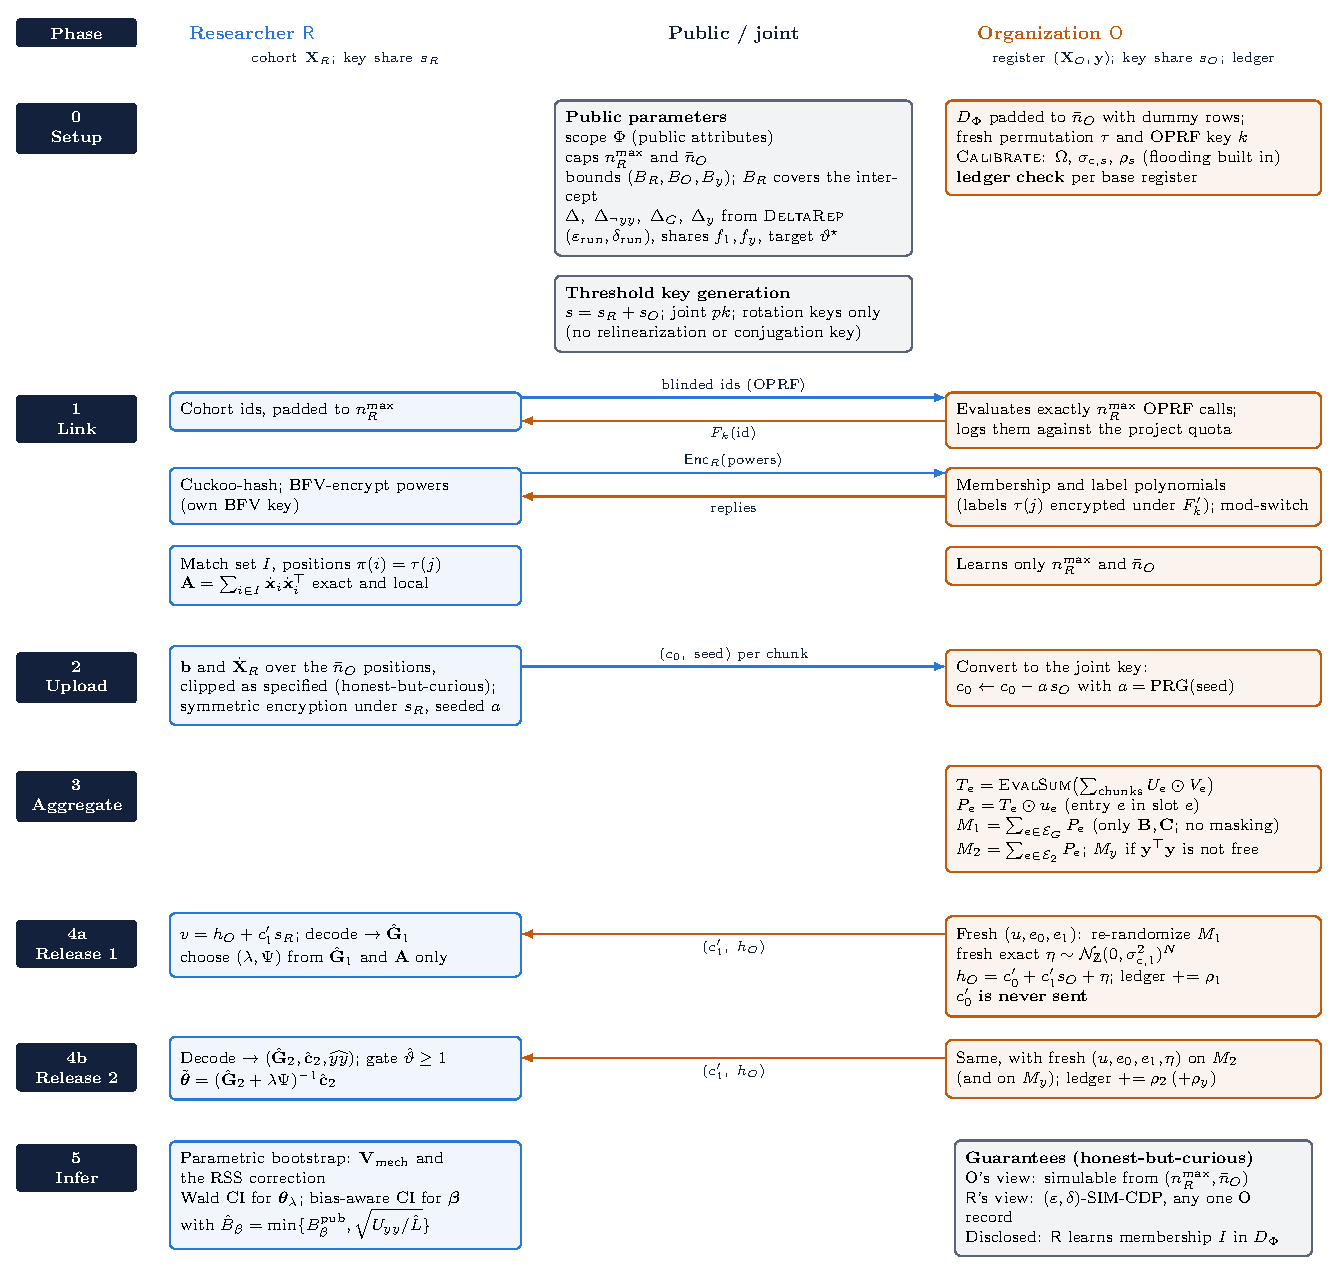
\includegraphics[width=\textwidth,height=0.92\textheight,keepaspectratio]{protocol_v31_fig.pdf}
  \caption{Message flow of protocol v3.1. Blue arrows go from $\Rp$ to $\Op$ and orange arrows from $\Op$ to $\Rp$. $\Op$ never receives a decryption share, and $\Rp$ never receives $c_0'$.}
  \label{fig:flow}
\end{figure}

Figure~\ref{fig:flow} shows the message flow. Algorithms~\ref{alg:setup}--\ref{alg:sub} give the details.

\begin{algorithm}[h]
\caption{Setup}\label{alg:setup}
\begin{algorithmic}[1]
\State \Bdo agree on the parameter vector $\mathcal P$ (Table~\ref{tab:params}): $\Phi$ (public attributes only), $n_R^{\max}$, $\bar n_O$, $(\varepsilon_{\mathrm{run}},\delta_{\mathrm{run}})$, the ledger parameters $(\varepsilon_L,\delta_L,\zeta_L,\xi_L,\delta')$, $f_1$ ($f_y$), $\zeta$, $\kappa_{\min}$ (or a fixed $\kappa$), $\delta_B$, $t_\eta$, $\vartheta^\star$, $\alpha_{\mathrm{CI}},\alpha_L,\alpha_U$, $B_\beta^{\mathrm{pub}}$, $\kappa_\Psi$, $\eta_B$, $B$, the PSI parameters, $N$, the chain, $\Omega_U$, $\Omega_u$
\State \Odo $D_\Phi\gets\{j:\Phi(j)\}$; pad with dummy rows to $\bar n_O$; draw a fresh secret permutation $\tau$ of $[\bar n_O]$
\State \Rdo and \Odo, each on its own columns only: \textsc{Preprocess} with constants from public reference data or domain knowledge
\State \Bdo $(B_R,B_O,B_y)\gets\textsc{ChooseBounds}$ on the preprocessed reference data, or from domain knowledge \Comment{$B_R$ covers the intercept}
\State $(\Delta,\Delta_{\neg yy})\gets\textsc{DeltaRep}(B_R,B_O,B_y)$;\quad $\Delta_G\gets\textsc{DeltaRep}(B_R,B_O,0)$;\quad $\Delta_y\gets B_y^2$
\State $\textit{mode}\gets\textsf{joint}$ if $\Delta-\Delta_{\neg yy}\le10^{-9}\Delta$, otherwise $\textsf{separate}$ \Comment{release $\by^\top\by$ jointly only when it is free}
\State \Odo $(\kappa,\Omega_V,\Omega_f,\{\sigma_{c,s},\rho_s\}_s,\mathit{cost})\gets\textsc{Calibrate}(\mathcal P)$; refuse if it refuses \Comment{Algorithm~\ref{alg:sub}; $\Rp$ repeats it}
\State \Odo atomically: \textbf{if} the ledger of the base register admits the run's cost $(\rho_{\mathrm{run}},\varepsilon'_{\mathrm{run}},\gamma_L)$ (Section~\ref{sec:ledger}) \textbf{then} charge it in full \textbf{else} refuse \Comment{no refund}
\State \Bdo threshold key generation (Mouchet et al., 2021) with a common random $a$: $s=s_R+s_O$, $pk=(p_0,a)$ with $p_0=-as+e$, and rotation keys for $\{2^i\}$
\Statex \hspace{\algorithmicindent}(no relinearization or conjugation key)
\State \Odo fresh OPRF key $k$; per-run PSI preprocessing on $\{F_k(\mathrm{id}_j)\}$ with labels $\tau(j)$ encrypted under $H(F'_k(\mathrm{id}_j))$
\Statex \hspace{\algorithmicindent} padding (bin degree, number of partitions) public; log the run against the quota for (researcher, project)
\end{algorithmic}
\end{algorithm}

\begin{algorithm}[h]
\caption{Link (labeled PSI with an OPRF)}\label{alg:link}
\begin{algorithmic}[1]
\State \Rdo pad the cohort identifiers with random dummies to exactly $n_R^{\max}$
\State \Rdo run the OPRF with $\Op$ on each padded identifier $\to F_k(\mathrm{id})$ \Comment{$\Op$ evaluates exactly $n_R^{\max}$ calls}
\State \Rdo cuckoo-hash the PRF values; send BFV encryptions of windowed powers under $\Rp$'s own BFV key
\State \Odo evaluate the membership and label polynomials per bin and partition; mask; \textsc{SanitizeBFV}; reply \Comment{flooding $\kappa_\psi$; abort if a sampler call fails}
\State \Rdo decrypt $\to$ the match set $I$ and positions $\pi(i)=\tau(j)$ for $i\in I$ (labels decrypted with keys from $F'_k(\mathrm{id})$); abort on an ambiguous or out-of-range position, or if two identifiers receive the same position
\State \Rdo $\bA\gets\sum_{i\in I}\bxd_i\bxd_i^\top$, exact and local
\end{algorithmic}
\end{algorithm}

\begin{algorithm}[h]
\caption{Upload}\label{alg:upload}
\begin{algorithmic}[1]
\For{$t=1,\dots,\bar n_O$}
  \State \Rdo $b_t\gets\mathbb{1}[t\in\pi(I)]$;\quad $\bxd_t\gets\bigl(1,\ \mathrm{clip}(\bx_{R,i};\sqrt{B_R^2-1})\bigr)$ if $t=\pi(i)$, otherwise $\mathbf 0$
\EndFor
\State $m\gets\lceil\bar n_O/N_s\rceil$
\For{each vector $\mathbf v\in\{\bb,\bxd_{\cdot0},\dots,\bxd_{\cdot d_R}\}$ and each chunk $h\le m$}
  \State \Rdo draw a seed $\varsigma$; $a\gets\mathrm{PRG}(\varsigma)$; $c_0\gets-a\,s_R+e+\Ecd_{\Omega_U}(\mathbf v[h])$, with $e$ from the RLWE error distribution; send $(c_0,\varsigma)$
  \State \Odo $a\gets\mathrm{PRG}(\varsigma)$;\ $c_0\gets c_0-a\,s_O$ \Comment{$(c_0,a)$ now encrypts $\mathbf v[h]$ under $s=s_R+s_O$}
\EndFor
\end{algorithmic}
\end{algorithm}

\begin{algorithm}[h]
\caption{Aggregate and pack ($\Op$)}\label{alg:aggregate}
\begin{algorithmic}[1]
\Require entry map $e\mapsto(U_e,V_e)$, with $\Rp$'s ciphertext vector $U_e$ and $\Op$'s plaintext vector $V_e$ in $\tau$-order:
\Statex \quad $\bB_{jk}$: $(\Enc(\bb),\ \bx_{O,j}\odot\bx_{O,k})$;\quad $\bC_{jk}$: $(\Enc(\bxd_j),\ \bx_{O,k})$;\quad $\bc_{R,j}$: $(\Enc(\bxd_j),\ \by)$;\quad $\bc_{O,k}$: $(\Enc(\bb),\ \bx_{O,k}\odot\by)$;\quad $\by^\top\by$: $(\Enc(\bb),\ \by\odot\by)$
\For{each $e\in\mathcal E$}
  \State $T_e\gets\textsc{EvalSum}\bigl(\textsc{Rescale}\bigl(\sum_{h\le m}U_e[h]\odot\Ecd_{\Omega_V}(V_e[h])\bigr)\bigr)$ \Comment{sum the chunks first; one \textsc{EvalSum} per entry}
  \State $P_e\gets\textsc{Rescale}\bigl(T_e\odot\Ecd_{\Omega_u}(\mathbf u_{\mathrm{slot}(e)})\bigr)$ \Comment{$\mathbf u_k$ = one-hot slot $k$; entry $e$ sits only in slot $\mathrm{slot}(e)$}
\EndFor
\State $M_1\gets\sum_{e\in\mathcal E_G}P_e$;\quad $M_2\gets\sum_{e\in\mathcal E_2}P_e$;\quad $M_y\gets P_{\by^\top\by}$ if $\textit{mode}=\textsf{separate}$
\State $M_1$, $M_2$, $M_y$ are now at $q_0$ (a modulus switch is a no-op after the two rescales) \Comment{depth 2; $M_1$ depends only on $\triu\bB$ and $\bC$}
\Statex Scales: $\Rp$'s vectors at $\Omega_U$, masks at $\Omega_u$ (parameters), $\Op$'s data at $\Omega_V$ (from \textsc{Calibrate}); $\Omega_f=\Omega_U\Omega_V\Omega_u/(q_1q_2)$ is tracked exactly
\end{algorithmic}
\end{algorithm}

\begin{algorithm}[h]
\caption{Release$(M,\sigma_c)$: one DP release}\label{alg:release}
\begin{algorithmic}[1]
\State \Odo sample fresh $u$ from the key distribution and $e_0,e_1$ from the error distribution
\State \Odo $c_0'\gets c_0+p_0u+e_0$;\quad $c_1'\gets c_1+au+e_1$ \Comment{re-randomize $M=(c_0,c_1)$ under the joint $pk$}
\State \Odo $\eta\gets\textsc{SampleDGBudget}(\sigma_c^2,N)$, fresh; \textbf{refuse} the release if it fails \Comment{exact on $\Z^N$; fixed work; fails w.p.\ $\le\xi_T$}
\State \Odo $h_O\gets c_0'+c_1's_O+\eta\bmod q_0$
\State \Odo send $(c_1',h_O)$; erase $c_0',u,e_0,e_1,\eta$ \Comment{$c_0'$ is never sent; the ledger was charged at admission}
\Statex \hspace{\algorithmicindent}(implementation, defence in depth: $\Op$ holds the reply until a public deadline after the request and refuses an overrun)
\State \Rdo $v\gets h_O+c_1's_R\bmod q_0$;\quad \Return $\Dcd(v)$ restricted to the slots of this release \Comment{exact final scale $\Omega_f$}
\end{algorithmic}
\end{algorithm}

\begin{algorithm}[h]
\caption{Solve and infer ($\Rp$)}\label{alg:solve}
\begin{algorithmic}[1]
\Require $\bA$, $n$, $p$, slot-domain s.d.\ $\sigma_1,\sigma_2,\sigma_y$; from $\mathcal P$: $\vartheta^\star$, $\alpha=\alpha_{\mathrm{CI}}+\alpha_L+\alpha_U$, $B_\beta^{\mathrm{pub}}$, $\kappa_\Psi$, bootstrap truncation $\eta_B$ and size $B$
\State $(\hat\bB_1,\hat\bC_1)\gets\textsc{Release}(M_1,\sigma_{c,1})$;\quad $\hat\bG_1\gets\begin{psmallmatrix}\bA&\hat\bC_1\\ \hat\bC_1^\top&\hat\bB_1\end{psmallmatrix}$
\State $r_1\gets\sigma_1\bigl(2\sqrt p+2\sqrt{\ln(1/\alpha_L)}\bigr)$ \Comment{$\Pr[\|\bG-\hat\bG_1\|_{\mathrm{op}}>r_1]\le\alpha_L$}
\State $\hat L\gets\max\{0,\ \lambda_{\min}(\hat\bG_1)-r_1\}$;\quad $g^\star\gets2\vartheta^\star\sigma_2\sqrt p$
\State $\lambda_I\gets\max\{0,\ g^\star+r_1-\lambda_{\min}(\hat\bG_1)\}$;\quad $\lambda_O\gets\min\{\lambda\ge0:\lambda_{\min}(\hat\bG_1+\lambda\PiO)\ge g^\star+r_1\}$ (bisection; $\infty$ if none)
\State $(\lambda,\Psi)\gets(\lambda_O,\PiO)$ if $\lambda_O\le\kappa_\Psi\lambda_I$, otherwise $(\lambda_I,\bI)$ \Comment{uses stage 1 and $\bA$ only}
\State $(\hat\bB_2,\hat\bC_2,\hat\bc_R,\hat\bc_O,\widehat{yy})\gets\textsc{Release}(M_2,\sigma_{c,2})$; if separate, $\widehat{yy}\gets\textsc{Release}(M_y,\sigma_{c,y})$
\State assemble $\hat\bG_2$ and $\hat\bc_2$;\quad $\hat\vartheta\gets\lambda_{\min}(\hat\bG_2+\lambda\Psi)/(2\sigma_2\sqrt p)$;\quad \textbf{if} $\hat\vartheta<1$ \textbf{then return} \textsf{refused}
\State $\tilde\bP\gets(\hat\bG_2+\lambda\Psi)^{-1}$;\quad $\tilde\btheta\gets\tilde\bP\hat\bc_2$ \Comment{the bias correction is an option}
\State $\widetilde{\mathrm{RSS}}\gets\widehat{yy}-\hat\bc_2^\top\tilde\btheta-\lambda\,\tilde\btheta^\top\Psi\tilde\btheta$
\For{$b=1,\dots,B$} \Comment{parametric bootstrap of the mechanism: post-processing}
  \State draw $\mathbf E^*$ (symmetric, s.d.\ $\sigma_2$ on the $\Op$-dependent entries, zero on $\bA$), $\mathbf f^*\sim\mathcal N(0,\sigma_2^2\bI)$, $g^*\sim\mathcal N(0,\sigma_{yy}^2)$
  \State \textbf{keep} the draw only if $\|\tilde\bP^{1/2}\mathbf E^*\tilde\bP^{1/2}\|_{\mathrm{op}}\le\eta_B$ \Comment{truncation: otherwise the moments do not exist}
  \State $\btheta^*_b\gets(\hat\bG_2+\mathbf E^*+\lambda\Psi)^{-1}(\hat\bc_2+\mathbf f^*)$;\quad $\mathrm{RSS}^*_b\gets$ the same RSS formula at $(\hat\bG_2+\mathbf E^*,\hat\bc_2+\mathbf f^*,\widehat{yy}+g^*)$
\EndFor
\State $\bV_{\mathrm{mech}}\gets\widehat{\mathrm{Cov}}_b(\btheta^*_b)$;\quad $\mathrm{Corr}\gets\overline{\mathrm{RSS}^*}-\widetilde{\mathrm{RSS}}$;\quad $\tilde s^2\gets\max\{\widetilde{\mathrm{RSS}}-\mathrm{Corr},0\}/(n-p)$
\State \textbf{CI for the protocol estimand} $\btheta_\lambda=(\bG+\lambda\Psi)^{-1}\bc$:\quad $\tilde\theta_j\pm z_{1-\alpha_{\mathrm{CI}}/2}\sqrt{(\bV_{\mathrm{mech}})_{jj}}$
\State $\bV\gets\bV_{\mathrm{mech}}+\tilde s^2\,\tilde\bP\hat\bG_2\tilde\bP$ \Comment{adds sampling variance under the homoskedastic linear model}
\State $U_{yy}\gets\widehat{yy}+z_{1-\alpha_U}\sigma_{yy}+B_y^2\sqrt{n\ln(1/\alpha_U)/2}$;\quad $\hat B_\beta\gets\min\{B_\beta^{\mathrm{pub}},\sqrt{U_{yy}/\hat L}\}$ \Comment{$\sqrt{\cdot}=\infty$ if $\hat L=0$}
\State $\bar b_j\gets\lambda\,\|\Psi\tilde\bP\mathbf e_j\|_2\,\hat B_\beta$ \Comment{worst-case ridge bias of coordinate $j$}
\State \textbf{CI for} $\beta_j$ (bias-aware; Armstrong, Kolesár and Kwon): $\tilde\theta_j\pm\mathrm{cv}_{\alpha_{\mathrm{CI}}}\bigl(\bar b_j/\sqrt{V_{jj}}\bigr)\sqrt{V_{jj}}$
\Statex \hspace{\algorithmicindent}where $\mathrm{cv}_\alpha(t)$ is the $(1-\alpha)$ quantile of $|Z+t|$, $Z\sim\mathcal N(0,1)$
\State \Return $\tilde\btheta$, both intervals, $(\lambda,\Psi)$, the shrinkage $-\lambda\tilde\bP\Psi\tilde\btheta$, $\hat\vartheta$, and $(\varepsilon,\delta)$ spent
\end{algorithmic}
\end{algorithm}

\begin{algorithm}[h]
\caption{Subroutines}\label{alg:sub}
\begin{algorithmic}[1]
\Function{DeltaRep}{$B_R,B_O,B_y$} \Comment{replace-one of $(\bx_O,y)$, $\bxd$ fixed; $r,o,w=B_R^2,B_O^2,B_y^2$}
  \State \textbf{if} $|r-w|\le2o$: $\Delta^2=(2o+r+w)^2/2+2rw$;\quad \textbf{else if} $r-w\ge2o$: $\Delta^2=4r(o+w)$
  \State \textbf{else}: one-dimensional maximization, rounded up. Return $\Delta$, and $\Delta_{\neg yy}$ from the same maximization without the $(y^2-y'^2)^2$ term
  \State \Comment{for $d_O\ge2$ these are exact suprema; $\Delta_G=\textsc{DeltaRep}(B_R,B_O,0)=(2o+r)/\sqrt2$ if $r\le2o$, otherwise $2\sqrt{ro}$}
\EndFunction
\Function{Calibrate}{$\mathcal P$} \Comment{public values only; refuses when a step has no solution}
  \State \textit{mode}, $n_{\mathrm{rel}}\in\{2,3\}$, $\{\Delta_s\}$ as in Setup;\quad \textbf{refuse if} $\log_2(QP)>L_{\max}(N,\lambda_{\mathrm{sec}})$
  \State $\gamma(k):=n_{\mathrm{rel}}\bigl(\delta_B+2^{-k}(1+2^{-80})+2^{-97}+\xi_T\bigr)$;\quad $\varepsilon'(k):=\min\{\varepsilon:\delta(\pi4^{-k},\varepsilon)\le\delta'\}$
  \State \textbf{unless} $\mathcal P$ fixes $\kappa$: $\kappa\gets\max\{\kappa_{\min},\kappa_{\mathrm{run}},\kappa_L\}$ \Comment{refuse if none exists}
  \Statex \hspace{\algorithmicindent}$\kappa_{\mathrm{run}}=\min\{k:(1+e^{\varepsilon_{\mathrm{run}}})\gamma(k)\le\zeta\delta_{\mathrm{run}}\}$;\quad $\kappa_L=\min\{k:n_{\mathrm{rel}}\varepsilon'(k)\le(\tilde\rho_{\mathrm{run}}/\rho_L)\,E'_L\}$;
  \Statex \hspace{\algorithmicindent}\textbf{refuse if} $n_{\mathrm{rel}}(\delta_B+\delta'+\xi_T)>(\tilde\rho_{\mathrm{run}}/\rho_L)\,\Gamma_L$ \Comment{$\rho_L$, $E'_L$, $\Gamma_L$: Section~\ref{sec:ledger}}
  \State $\gamma\gets\gamma(\kappa)$;\quad $\delta_{\mathrm{DP}}\gets\delta_{\mathrm{run}}-(1+e^{\varepsilon_{\mathrm{run}}})\gamma$;\quad \textbf{refuse if} $\delta_{\mathrm{DP}}\le0$
  \State $\rho_{\mathrm{run}}\gets\max\{\rho:\ \inf_{a>1}\frac{e^{(a-1)(a\rho-\varepsilon_{\mathrm{run}})}}{a-1}\bigl(1-\tfrac1a\bigr)^{a}\le\delta_{\mathrm{DP}}\}$ \Comment{tight zCDP conversion (Canonne et al., 2020)}
  \State $\rho_1\gets f_1\rho_{\mathrm{run}}$;\quad $\rho_y\gets f_y\rho_{\mathrm{run}}$ (0 in joint mode);\quad $\rho_2\gets\rho_{\mathrm{run}}-\rho_1-\rho_y$
  \For{$\Omega_f$ in increasing admissible scales} \Comment{$\Omega_V=\Omega_fq_1q_2/(\Omega_U\Omega_u)$, exactly representable}
    \State for each release $s$: $\widehat\Delta_{\mathrm{enc},s}\gets\sqrt{2/N}\,\Omega_f\Delta_s+\Delta_{x,s}+\sqrt N$;\quad $\sigma_{c,s}^2\gets\lceil\widehat\Delta_{\mathrm{enc},s}^2/(2\rho_s)\rceil$
    \State \textbf{if} $\sigma_{c,s}\ge\max\{2^{\kappa}B_{\mathrm{tot},s}(\Omega_f)/\sqrt{2\pi},2^{42}\}$ for every $s$ \textbf{then break} \Comment{worst-case $B_{\mathrm{tot},s}$}
  \EndFor \Comment{refuse if no scale floods}
  \State $\sigma_s\gets\sigma_{c,s}\sqrt{N/2}/\Omega_f$;\quad \textbf{refuse unless} $q_0>2\bigl(\Omega_fS_{\max}+2^{\kappa}B_{\mathrm{tot},\max}+t_\eta\sigma_{c,\max}\bigr)$
  \Statex \hspace{\algorithmicindent}with $S_{\max}=\bar n_O\max(r,o,w,\sqrt{ro},\sqrt{rw},\sqrt{ow})$ \Comment{no wraparound}
  \State $T_s\gets$ the work budget of \textsc{SampleDGBudget}$(\sigma_{c,s}^2,N)$ at $\xi_T$ \Comment{public; checked by $\Rp$}
  \State \Return $\kappa$, $\Omega_V$, $\Omega_f$, $\{\sigma_{c,s}^2,\sigma_s,\rho_s,T_s\}_s$, and the run's ledger cost $\mathit{cost}=(\rho_{\mathrm{run}},\ n_{\mathrm{rel}}\varepsilon'(\kappa),\ n_{\mathrm{rel}}(\delta_B+\delta'+\xi_T))$
\EndFunction
\Function{SampleDGBudget}{$\sigma^2,n$} $n$ exact samples of $\DG(0,\sigma^2)$, integer $\sigma^2$, with a fixed work budget; never by rounding a floating-point normal
  \State $t\gets2^b\approx\sigma$;\quad $c\gets\lceil2^{128}\sigma^2/(2t^2)\rceil/2^{128}$;\quad $(T,J_v,k_{\max})$ from $(\sigma^2,n,\xi_T)$ \Comment{public}
  \For{$j=1,\dots,T$, all of them, with the same fixed-width operations} \Comment{coins: 128-bit uniforms from a CSPRNG}
    \State $s\gets$ bit;\ $u\gets\mathrm U[0,t)$;\ $v\gets\#\{1\le i\le J_v:U<e^{-i}\}$;\ $y_j\gets u+tv$ if $s=0$, else $-(u+tv+1)$
    \State $g\gets y_j^2/(2\sigma^2)-v+c\ (\ge0)$;\ $a_j\gets\mathrm{Bern}(e^{-\lfloor g\rfloor})\wedge\mathrm{Bern}(e^{-\{g\}})$ \Comment{the latter: CKS20 Alg.~1 with exactly $k_{\max}$ coins}
  \EndFor
  \State \textbf{fail} if some trial is undecided ($v=J_v$, all $k_{\max}$ coins $1$, or a coin equal to its threshold) or $\sum_ja_j<n$
  \State \Return the first $n$ values $y_j$ with $a_j=1$ \Comment{$\Pr[\textbf{fail}]\le\xi_T$ (Proofs, Part~A, Sec.~5.5)}
\EndFunction
\Function{SanitizeBFV}{$\mathit{ct}$} \Comment{statistical flooding of a PSI reply; BFV decryption stays exact}
  \State $\mathit{ct}\gets\mathsf{ModSwitch}_{q'}(\mathit{ct})\boxplus\mathsf{ModSwitch}_{q'}\bigl(\mathsf{BFV.Enc}_{pk_B}(\mathbf 0)\bigr)$;\quad $\mathbf e\gets\textsc{SampleDGBudget}(\sigma_\psi^2,N_B)$ \Comment{$\sigma_\psi\ge\max\{2^{\kappa_\psi}B_\psi/\sqrt{2\pi},2^{42}\}$}
  \State \Return $\mathit{ct}\boxplus(\mathbf e,0)$ \Comment{requires $q'/(2t)>t_\eta\sigma_\psi+B_\psi+t$}
\EndFunction
\Function{Preprocess}{own columns, $D_{\mathrm{ref}}$} \Comment{each party separately; all constants public}
  \State standardize each column with constants from $D_{\mathrm{ref}}$ or domain knowledge ($\Op$ also standardizes $y$)
  \State optional tail transform per column: winsorize at $|z|\le c$, rank-Gaussian from the public quantiles, or log
  \State optional block normalization: scale the party's block of every row to unit norm ($\Rp$ without the intercept)
\EndFunction
\Function{ChooseBounds}{$D_{\mathrm{ref}}$} grid over quantile levels of $\|\bxd\|$, $\|\bx_O\|$ and $|y|$ in the preprocessed reference data; minimize
\Statex \hspace{\algorithmicindent}the first-order coefficient MSE plus the squared clipping bias (for block normalization the bounds are exact: $B_R^2=2$, $B_O=1$)
\EndFunction
\end{algorithmic}
\end{algorithm}

% ==============================================================
\section{The release mechanism and output privacy}
\label{sec:privacy}

\paragraph{Encoded statistic and centre.} For release $s$, let $\mathbf z_s(D)\in\mathbb R^{N_s}$ hold the released entries in their slots and zeros elsewhere. The mechanism is centred at the noiseless circuit output $f_s(D)=\lfloor\hat{\mathbf z}_s(D)\rceil\in\Z^N$, with $\hat{\mathbf z}_s(D)=\sum_{e\in\mathcal E_s}(q_1q_2)^{-1}\mathrm{Tr}\bigl(\sum_hm_{U_e,h}m_{V_e,h}\bigr)m_{u_e}$, where $m_{U_e,h}$, $m_{V_e,h}$, $m_{u_e}$ are the encodings at $\Omega_U$, $\Omega_V$, $\Omega_u$. $f_s$ depends on the data and public parameters only. It differs from $\Ecd_{\Omega_f}(\mathbf z_s(D))$ by deterministic terms, chiefly the mask spill, which are part of the query and need no flooding.

\begin{lemma}[Sensitivity of the encoded statistic and of the centre]\label{lem:enc}
$\|\tau^{-1}(\mathbf z)\|_2=\sqrt{2/N}\,\|\mathbf z\|_2$, so $\sup_{D\sim D'}\|\Ecd_\Omega(\mathbf z_s(D))-\Ecd_\Omega(\mathbf z_s(D'))\|_2\le\sqrt{2/N}\,\Omega\,\Delta_s+\sqrt N$. For the centre (proofs, Part~A),
\[
  \sup_{D\sim D'}\|f_s(D)-f_s(D')\|_2\le\widehat\Delta_{\mathrm{enc},s}:=\sqrt{2/N}\,\Omega_f\Delta_s+\Delta_{x,s}+\sqrt N,
\]
with $\Delta_{x,s}$ an explicit function of $N$, the scales, $q_1,q_2$, $|\mathcal E_s|$, the bounds and $\Delta_s$. $\Omega_f$ is the exact final scale, tracked exactly; $\Rp$ decodes with it.
\end{lemma}

\paragraph{Error decomposition.} Write the value $\Rp$ reconstructs in Algorithm~\ref{alg:release} as
\[
  v_s=h_O+c_1's_R=c_0'+c_1's+\eta=f_s(D)+e_{\mathrm{tot},s}+\eta_s\pmod{q_0}.
\]
$e_{\mathrm{tot},s}\in\Z^N$ collects every term that depends on a key, an error or a coin: $\Rp$'s encryption errors times $\Op$'s data, the rescaling and ModDown roundings, the key-switching error (which involves $\Op$'s key-share errors), the mask spill of these errors, the rounding of the centre, and the fresh-encryption error $e\,u+e_0+e_1s$.

\begin{obligation}[Worst-case error bound; discharged in the proofs, Part~A, Theorem~O1]\label{obl:err}
For the circuit of Algorithm~\ref{alg:aggregate}, $B_{\mathrm{tot},s}$ is an explicit function of public parameters only ($N$, $\bar n_O$, $d_R$, $d_O$, the bounds, the primes and the key-switching gadget, $\Omega_U,\Omega_V,\Omega_u$, $\delta_B$, the error distribution) with $\Pr[\|e_{\mathrm{tot},s}\|_2\le B_{\mathrm{tot},s}]\ge1-\delta_B$ for every dataset $D$ in the clipped domain, the probability being over the keys and fresh randomness only. \textsc{Calibrate} must use this worst-case bound, never a value estimated from the ciphertexts.
\end{obligation}

\begin{lemma}[Smudging]\label{lem:smudge}
If $\eta\sim\DG(0,\sigma_c^2)^N$, $\sigma_c\ge\max\{2^{\kappa}B_{\mathrm{tot}}/\sqrt{2\pi},2^{42}\}$ and $\|e\|_2\le B_{\mathrm{tot}}$, then $\mathrm{SD}(\eta+e,\eta)\le2^{-\kappa}(1+2^{-80})+2^{-97}$, also given side information independent of $\eta$.
\end{lemma}

\begin{theorem}[Output privacy against an honest-but-curious $\Rp$]\label{thm:output}
Let $\mathcal P$ be admissible (Section~\ref{sec:params}), let every release draw its noise with \textup{\textsc{SampleDGBudget}} at failure bound $\xi_T$, and let \textup{\textsc{Calibrate}}'s outputs satisfy $\sigma_{c,s}\ge\max\{2^{\kappa}B_{\mathrm{tot},s}/\sqrt{2\pi},2^{42}\}$, $\rho_s=\widehat\Delta_{\mathrm{enc},s}^2/(2\sigma_{c,s}^2)$ and $\sum_s\rho_s\le\rho_{\mathrm{run}}$, where $\rho_{\mathrm{run}}$ converts to $(\varepsilon_{\mathrm{run}},\delta_{\mathrm{DP}})$ and
\[
  \gamma=n_{\mathrm{rel}}\bigl(\delta_B+2^{-\kappa}(1+2^{-80})+2^{-97}+\xi_T\bigr),\qquad \delta_{\mathrm{DP}}=\delta_{\mathrm{run}}-(1+e^{\varepsilon_{\mathrm{run}}})\gamma>0 .
\]
Assume RLWE for the re-randomizer (one sample per release, modulus $q_0$) and for $\Op$'s key shares (multi-sample, with circular security for the rotation-key shares; Mouchet et al., 2021), with $\log_2(QP)\le L_{\max}(N,\lambda_{\mathrm{sec}})$. Assume (W): the duration of a fixed sequence of operations of $\Op$ on fixed-shape operands does not depend on the operand values (machine noise aside). Then $\Rp$'s view of one run, including the time at which each release (or refusal) arrives, is $(\varepsilon_{\mathrm{run}},\delta_{\mathrm{DP}})$-SIM-CDP for $\sim$ with slack $\gamma$, hence $(\varepsilon_{\mathrm{run}},\delta_{\mathrm{run}})$-IND-CDP. The ideal mechanism $\mathcal M(D)=(f_s(D)+\eta_s)_s$ is $\rho_{\mathrm{run}}$-zCDP. PSI security is not needed: the identifiers are fixed under $\sim$, so the PSI transcript does not depend on $(\bx_O,y)$.
\end{theorem}

\begin{proof}[Proof sketch]
\textbf{H0} is the real view. \textbf{H0}$'$ replaces each release's noise by the unbudgeted exact sampler's output on the same coins and its timing by that of the sampler's fixed operation sequence: they differ only when the call fails, so this costs $\xi_T$ per release; under (W) the timing is then independent of $\eta_s$ and of the data. \textbf{H1} rewrites $h_{O,s}=v_s-c'_{1,s}s_R$ (identical). \textbf{H2} replaces $v_s$ by $f_s(D)+\eta_s$; by Lemma~\ref{lem:smudge} and Obligation~\ref{obl:err} this costs at most $\delta_B+2^{-\kappa}(1+2^{-80})+2^{-97}$ per release; with H0$'$, $\gamma$ in total. After H2, $(u_s,e_{1,s})$ appear only through $c'_{1,s}=c_{1,s}+au_s+e_{1,s}$, because $c'_{0,s}$ is never sent. \textbf{H3} replaces $c'_{1,s}$ by a uniform element (RLWE with secret $u_s$, fresh per release). \textbf{H4} simulates the setup messages from RLWE on $\Op$'s key shares. The multivariate discrete Gaussian with sensitivity $\widehat\Delta_{\mathrm{enc},s}$ is exactly $\rho_s$-zCDP (Canonne et al., 2020); costs add; the tight conversion gives $(\varepsilon_{\mathrm{run}},\delta_{\mathrm{DP}})$-DP, and SIM-to-IND adds $(1+e^{\varepsilon_{\mathrm{run}}})\gamma$.
\end{proof}

\begin{remark}[Why the release format matters]
If $\Op$ sent $c_0'$, or a share $c_1's_O$ without $\eta$, then $\Rp$ would learn $c_1's_O$ exactly and could recover $s_O$, since $c_1'$ is invertible with overwhelming probability. That was critical issue C3. Sending $h_O=c_0'+c_1's_O+\eta$ and $c_1'$ only means that everything $\Rp$ learns is a function of the noisy value $v_s$ and of $c_1'$, which is pseudorandom. Reusing $\eta$ or $u$ across releases would reveal $v_2-v_1$ exactly, so both are fresh every time. Stage~1 uses its own packed ciphertext $M_1$, which depends only on $\triu\bB$ and $\bC$.
\end{remark}

\paragraph{Calibrate.} \textsc{Calibrate} (Algorithm~\ref{alg:sub}) derives, from public values only: the mode and $n_{\mathrm{rel}}$; the flooding parameter and the slack; $\rho_{\mathrm{run}}$ and its split; the smallest admissible $\Omega_f$ (that is, $\Omega_V$) at which every $\sigma_{c,s}^2=\lceil\widehat\Delta_{\mathrm{enc},s}^2/(2\rho_s)\rceil$ floods; and it checks $q_0>2(\Omega_fS_{\max}+2^{\kappa}B_{\mathrm{tot},\max}+t_\eta\sigma_{c,\max})$ and $\log_2(QP)\le L_{\max}(N,\lambda_{\mathrm{sec}})$ (Homomorphic Encryption Security Standard, 2018). It refuses the run when a step has no solution.

\paragraph{The flooding parameter.} The flooding enters the guarantee only through $\gamma$, which the SIM-to-IND step multiplies by $1+e^{\varepsilon}$. Unless $\mathcal P$ fixes it,
\[
  \kappa=\max\{\kappa_{\min},\kappa_{\mathrm{run}},\kappa_L\},
\]
where $\kappa_{\mathrm{run}}$ is the smallest integer with $(1+e^{\varepsilon_{\mathrm{run}}})\gamma\le\zeta\delta_{\mathrm{run}}$; $\kappa_L$ is the smallest with $n_{\mathrm{rel}}\varepsilon'(\kappa)\le(\tilde\rho_{\mathrm{run}}/\rho_L)E'_L$, the run's share of the ledger's smudging budget, with $\tilde\rho_{\mathrm{run}}$ the budget at $\delta_{\mathrm{DP}}=(1-\zeta)\delta_{\mathrm{run}}$ (it holds whenever the zCDP condition does, provided every run uses $\kappa\ge\kappa_L$); and $\kappa_{\min}$ is a statistical security floor. $\kappa_{\mathrm{run}}$ exists iff $n_{\mathrm{rel}}(1+e^{\varepsilon_{\mathrm{run}}})(\delta_B+2^{-97}+\xi_T)<\zeta\delta_{\mathrm{run}}$. $\zeta$ trades budget for bits: it lowers $\rho_{\mathrm{run}}$ by a relative $\zeta/\sqrt{L(L+\varepsilon_{\mathrm{run}})}$ to first order, $L=\ln(1/\delta_{\mathrm{run}})$, while each unit of $\kappa$ costs one bit of $\Omega_f$ and of $q_0$.

\paragraph{Encoding scales.} $\Omega_U$ and $\Omega_u$ are parameters, $\Omega_V$ is chosen by \textsc{Calibrate}, and $\Omega_f$ follows. The term of $B_{\mathrm{tot}}$ from $\Rp$'s encryption errors grows like $(\Omega_f/\Omega_U)\sqrt{\bar n_O}$; with $\Omega_U\ge\Omega_f$ it does not grow with the register, otherwise the required scale grows with $\bar n_O$ and, for large $\kappa$, no scale floods.

\subsection*{Ledger and composition across runs}
\label{sec:ledger}
$\Op$ keeps one ledger per base register, shared across all researchers and scopes; it admits a run only if the run's full cost fits under the cap and produces decryption shares only within admitted runs, so the cap is enforced technically. Its parameters are a cap $(\varepsilon_L,\delta_L)$, a slack share $\zeta_L$, a share $\xi_L$ of $\varepsilon_L$ reserved for smudging, and a per-release constant $\delta'$ (evaluation: $\xi_L=10^{-3}$, $\delta'=2^{-100}$). With $\delta(\rho,\varepsilon)$ the tight conversion, $E'_L=\xi_L\varepsilon_L/2$, $\rho_L=\max\{\rho:\delta(\rho,(1-\xi_L)\varepsilon_L)\le e^{-E'_L}(1-\zeta_L)\delta_L\}$ and $\Gamma_L=\zeta_L\delta_L/(1+e^{\varepsilon_L-E'_L})$, each rounded down. A run costs $\rho_{\mathrm{run}}$, a smudging cost $\varepsilon'_{\mathrm{run}}=n_{\mathrm{rel}}\varepsilon'(\kappa)$ with $\varepsilon'(\kappa)=\min\{\varepsilon:\delta(\pi4^{-\kappa},\varepsilon)\le\delta'\}\le2\sqrt{\pi\ln(1/\delta')}\,2^{-\kappa}+\pi4^{-\kappa}$, and a slack $\gamma_L=n_{\mathrm{rel}}(\delta_B+\delta'+\xi_T)$; the state is the three sums $(\rho_\Sigma,E_\Sigma,\Gamma_\Sigma)$ over admitted runs. The full cost of a run, for all its planned releases, is charged atomically at admission and never refunded (refunding the $\delta_B$ part of an aborted run would not be sound); requests are processed one at a time. With $x^+$ the sum after adding the run: runs fixed in advance (parameters and inputs of every run fixed before the first) are admitted iff $e^{E^+}\delta(\rho^+,\varepsilon_L-2E^+)+(1+e^{\varepsilon_L-E^+})\Gamma^+\le\delta_L$; runs chosen after seeing earlier results are admitted iff $\rho^+\le\rho_L$, $E^+\le E'_L$ and $\Gamma^+\le\Gamma_L$ (a privacy filter, Rogers, Roth, Ullman and Vadhan, 2016). A single-run register is covered by Theorem~\ref{thm:output} alone, with cap $(\varepsilon_{\mathrm{run}},\delta_{\mathrm{run}})$. The OPRF quota limits membership look-ups across sessions as a matter of policy.

\begin{proposition}[Composition across runs]\label{prop:compose}
Let all researchers on a base register act as one PPT coalition, possibly colluding, that chooses each run's parameters and cohort from the joint view of earlier runs, follows the protocol within each run, and may interleave and abort runs. If every admitted run draws fresh key material and release coins and satisfies Theorem~\ref{thm:output}, the register is static, RLWE holds for every ring parameter set of a finite menu against non-uniform adversaries, and $\Op$'s ledger is honest, admits runs one at a time and charges a run's full cost at admission, then the joint view of all researchers is $(\varepsilon_L,\delta_L)$-IND-CDP for base-register adjacency (same identifiers and public attributes, one row's $(\bx,y)$ changed): under the filter rule for every coalition, and under the first rule when the runs are fixed in advance.
\end{proposition}
\begin{proof}[Proof sketch]
Proofs, Part~C (Theorems~4.2 and~5.2, Corollary~5.4). One statistical hybrid removes the encryption error from every release of every run, before any computational step; measured in hockey-stick divergence, each release costs $(\varepsilon'(\kappa),\delta')$, and $\delta_B$ is charged for every planned release of every admitted run. Computational hybrids then replace each run's $c_1'$ and key shares run by run. The ideal experiment is $\rho_L$-zCDP by a R\'enyi filter proved there. The conversion at $\varepsilon=(1-\xi_L)\varepsilon_L$ gives $(\varepsilon_L,\delta_L)$. Not proved: the first rule with adaptively chosen requests.
\end{proof}

\section{Input privacy and cohort privacy}

\paragraph{G1.} $\Op$ sees:
\begin{itemize}[nosep]
  \item $\Rp$'s uploads $c_0=-as_R+e+\Ecd(\mathbf v)$ with $a$ derived from a seed. These are pseudorandom under RLWE in $s_R$, modelling the PRG as a random oracle.
  \item The PSI messages, which are BFV ciphertexts under $\Rp$'s own key, and blinded OPRF queries.
  \item $\Rp$'s key-generation shares, which are RLWE samples.
\end{itemize}
$\Op$ never receives a decryption share from $\Rp$, so its view is simulable from $(n_R^{\max},\bar n_O)$.

\paragraph{G2.} $\Op$ evaluates exactly $n_R^{\max}$ OPRF calls on blinded inputs and answers padded PSI queries, so it learns nothing about the cohort or $n_R$.

\paragraph{G4.} $\Rp$ learns $I$ and $\pi|_I$; that it learns nothing else needs the labeled PSI to be secure against a semi-honest receiver, which Chen, Laine and Rindal (2017) base on IND-CPA security and circuit privacy (statistical function privacy, by re-randomization and noise flooding, suffices). Two layers address the noise of the replies. (a) Every item is $F_k(\mathrm{id}_j)$ under a fresh OPRF key and every label is $\tau(j)$ masked by a key derived from $F'_k(\mathrm{id}_j)$; $\Rp$ learns $F_k$ only at its queries, so items and labels outside $I$ are pseudorandom to it, and a simulator that knows $(I,\pi|_I)$ can rerun $\Op$'s evaluation on random items and labels outside $I$: the noise reveals nothing beyond pseudorandom values, under the OPRF's security (OPRF preprocessing, Chen, Huang, Laine and Rindal, 2018). (b) \textsc{SanitizeBFV} is part of the protocol nevertheless: switch the reply and a fresh encryption of zero to the reply modulus $q'$, add them, and flood with $\mathcal D_{\Z^{N_B},\sigma_\psi}$, where $B_\psi$ bounds, with probability $\ge1-\delta_{B,\psi}$ and for every input of $\Op$, the switched reply's error other than the flooding noise and an integral function $\varphi(m)$ of the plaintext with $\|\varphi(m)\|_\infty\le t/2+1$. Requirements: $\sigma_\psi\ge\max\{2^{\kappa_\psi}B_\psi/\sqrt{2\pi},2^{42}\}$ and $q'/(2t)>t_\eta\sigma_\psi+B_\psi+t$, the last term covering $\varphi(m)$. Either order of the switch and the addition supports the argument (switching both gives two rounding terms, which $B_\psi$ must cover); this is the implementation's order. Each reply is then within statistical distance $\delta_{B,\psi}+2^{-\kappa_\psi}(1+2^{-80})+2^{-97}$, plus an RLWE term, of a ciphertext computed from its plaintext alone. The flooding vectors come from \textsc{SampleDGBudget}, so under (W) the replies' timing adds at most $\xi_T$ per flooding vector ($2\alpha F$ per cuckoo table; \textsc{Setup} checks that the total is at most $\delta_{\mathrm{psi}}$) and a failed call aborts the run. Neither layer is charged to $\delta$. A worst-case bound on the BFV evaluation noise inside $B_\psi$ is still open; the implementation's value is measured.

\paragraph{Correctness.} With $q_0$ from \textsc{Calibrate}, honest inputs never wrap around, except with probability at most $\delta_B+2Ne^{-t_\eta^2/2}$ per release, a correctness event not charged to $\delta$.

% ==============================================================
\section{Parameters}
\label{sec:params}

The protocol is defined for a parameter vector $\mathcal P$; Table~\ref{tab:params} lists each parameter with its constraint and the evaluation setting of the paper and the implementation, which is one admissible choice and not part of the protocol. \textsc{Calibrate} checks the constraints that involve derived quantities and refuses otherwise.

{\small
\begin{longtable}{@{}>{\raggedright\arraybackslash}p{3.1cm}>{\raggedright\arraybackslash}p{7.6cm}>{\raggedright\arraybackslash}p{4.4cm}@{}}
\caption{Parameters, constraints and evaluation settings.}\label{tab:params}\\
\toprule
Parameter & Constraint & Evaluation setting \\
\midrule
\endfirsthead
\toprule
Parameter & Constraint & Evaluation setting \\
\midrule
\endhead
\bottomrule
\endlastfoot
$N$, chain $q_0,q_1,q_2$, $P$, $d_{\mathrm{num}}$, $\lambda_{\mathrm{sec}}$ & $\log_2(QP)\le L_{\max}(N,\lambda_{\mathrm{sec}})$ (438 for $N=2^{14}$ at 128 bits); $q_0$ above the no-wraparound bound & $N=2^{14}$; primes 60, 59 ($q_0$), 59, 59; $P$ two 60-bit primes; $d_{\mathrm{num}}=2$; $\log_2(QP)=357$ \\
$\delta_B$ & $n_{\mathrm{rel}}(1+e^{\varepsilon_{\mathrm{run}}})(\delta_B+2^{-97}+\xi_T)<\zeta\delta_{\mathrm{run}}$; $n_{\mathrm{rel}}(\delta_B+\delta'+\xi_T)$ below each run's ledger share & $2^{-50}$ \\
$\xi_T$ & failure bound per call of \textsc{SampleDGBudget}, charged per release in $\gamma$ & $2^{-80}$ \\
$\kappa_{\min}$; $\kappa$ & integer floor; $\kappa$ derived (or fixed with $\delta_{\mathrm{DP}}>0$) & $40$; derived \\
$t_\eta$ & $>0$; correctness failure $2Ne^{-t_\eta^2/2}$ per release & $10$ \\
$(\varepsilon_{\mathrm{run}},\delta_{\mathrm{run}})$ & admitted by the ledger & $\varepsilon\in\{0.5,1,2,4,8\}$, $\delta=10^{-9}$ \\
$f_1$; $f_y$ & $f_1\in(0,1)$; $f_y\in(0,1-f_1)$, separate mode only, no default & $0.1$; $0.1$ \\
$\zeta$ & $(0,1)$ & $0.1$ \\
$(\varepsilon_L,\delta_L)$, $\zeta_L$, $\xi_L$, $\delta'$, admission rule & public cap per base register, shares in $(0,1)$; filter rule unless runs are fixed in advance; full cost charged at admission & one run per register; example $(10,10^{-6})$, $\zeta_L=0.1$, $\xi_L=10^{-3}$, $\delta'=2^{-100}$ \\
$\vartheta^\star$; $\kappa_\Psi$ & $\vartheta^\star>1$ ($>2$ for the refusal bound); $\kappa_\Psi\ge0$ & $2.5$; $2$ \\
$\alpha_{\mathrm{CI}},\alpha_L,\alpha_U$ & positive, sum $\alpha<1$ & $0.045$, $0.0025$, $0.0025$ \\
$\eta_B$; $B$ & $\eta_B\in(0,1)$; Monte Carlo error $O(B^{-1/2})$ & $1/2$; $2000$ \\
$B_\beta^{\mathrm{pub}}$; bias correction & $>0$ or $\infty$; on or off & $\infty$; off \\
$B_R,B_O,B_y$; preprocessing & public, fixed in advance; per-party transforms with public constants & $99.5\%$ reference quantiles; standardize, optionally winsorize or block-normalize \\
$\Phi$, $\bar n_O$, $n_R^{\max}$ & public attributes only; public sizes & -- \\
$N_B$, $t$, $h$, $N_{\mathrm{bins}}$, $d_{\mathrm{cap}}$, $\delta_{\mathrm{psi}}$ & $t$ prime, $t\equiv1\bmod 2N_B$, $t-1\ge n_R^{\max}\bar n_Oh/(N_{\mathrm{bins}}\delta_{\mathrm{psi}})$ & $2^{14}$, $\approx2^{32}$ (does not meet the last constraint), $3$, $2^{14}$, $64$, $2^{-40}$ \\
$\kappa_\psi$, $B_\psi$, $\delta_{B,\psi}$, $q'$ & flooding and exact-decryption requirements of G4 & $40$; $2^{21}$ (evaluation noise measured); $0$; $2\times60$ bits \\
$\Omega_U$; $\Omega_u$; $\Omega_V$, $\Omega_f$ & exactly representable; $\Omega_U\ge\Omega_f$ keeps $B_{\mathrm{tot}}$ independent of $\bar n_O$; $\Omega_V$, $\Omega_f$ derived & $2^{68}$; $q_1$; derived \\
\end{longtable}}

\paragraph{Evaluation settings, derived values.} For the simulation population ($B_R=5.59$, $B_O=6.24$, $B_y=2.89$, $\Delta=86.15$, $\Delta_G=77.16$, joint mode) at $\delta=10^{-9}$ and a single-run ledger, \textsc{Calibrate} gives $\kappa=40,40,40,41,46$ for $\varepsilon=0.5,1,2,4,8$, with $\Omega_f=2^{61.78}$, $2^{62.75}$, $2^{63.69}$, $2^{65.62}$--$2^{65.66}$ and $2^{71.56}$--$2^{71.94}$ for $\bar n_O$ from $4{,}096$ to $10^6$; $q_0$ needs at most $98.2$ of its $119$ bits. At $\varepsilon=1$: $\sigma_2\approx525$, $\sigma_1\approx1410$, $B_{\mathrm{tot},2}\approx2^{26.6}$ with OpenFHE's key switching. Under a ledger cap $(10,10^{-6})$ with $\zeta_L=0.1$ and $\xi_L=10^{-3}$, $\kappa_L=22,21,19,17,15$, so $\kappa=40,40,40,41,46$ as for a single run (the statistical-distance accounting gave $\kappa_L=48,46,44,42,40$ and $\kappa=48,46,44,42,46$).

\paragraph{Cost.} Table~\ref{tab:cost} gives the cost per run.
\begin{table}[h]
\centering\small
\begin{tabularx}{\textwidth}{@{}l>{\raggedright\arraybackslash}X>{\raggedright\arraybackslash}X l@{}}
\toprule
Step & Communication & $\Op$'s computation & Rounds \\
\midrule
Link & $n_R^{\max}$ OPRF calls; PSI query and response (sublinear in $\bar n_O$) & per-run preprocessing $O(\bar n_O)$; per-query evaluation & 2--3 \\
Upload & $(d_R+2)\,m$ seeded ciphertexts (half size) & $(d_R+2)\,m$ conversions & 1 \\
Aggregate & -- & $|\mathcal E|\,m$ ct--pt products; $|\mathcal E|\log_2N_s$ rotations; $|\mathcal E|$ mask products & -- \\
Release ($\times2$ or $3$) & 2 ring elements each & 1 re-randomization, 1 partial decryption, $N$ exact samples & 2--3 \\
\bottomrule
\end{tabularx}
\caption{Cost per run, with $m=\lceil\bar n_O/N_s\rceil$. $\Op$'s computation is $\Omega(\bar n_O)$, which is inherent for oblivious selection; the public scope $\Phi$ is the main lever on it.}\label{tab:cost}
\end{table}

% ==============================================================
\section{Extensions and limitations}
\label{sec:ext}

\paragraph{A deviating researcher.} v3.1 makes no claim against a malicious $\Rp$. Making G3 hold against one requires:
\begin{enumerate}[nosep,label=(\roman*)]
  \item zero-knowledge proofs at upload that the ciphertexts are well formed with short errors, and that $b_t\in\{0,1\}$, $\|\bxd_t\|\le B_R$, $(1-b_t)\bxd_t=\mathbf0$, $\sum_tb_t\le n_R^{\max}$, together with a coarse norm bound that rules out wraparound. Candidates include lattice proofs (LNP22, LaBRADOR) and VOLE-based proofs;
  \item key generation with $\Rp$ committing first, plus proofs that its shares are short;
  \item OPRF inputs bound to a certified cohort.
\end{enumerate}
A homomorphic check that relies on $\Rp$'s own decryption share cannot do this job; that was critical issue C1.

\begin{remark}[Mode M: hiding membership]\label{rem:modeM}
Replacing labeled PSI with circuit-PSI (e.g.\ VOLE-PSI with payloads) gives both parties shares of $\bb$ and $\dot\bX_R$ in $\tau$-order, so $\Rp$ no longer learns $I$. The aggregation would move to BFV or use wide statistical masking, because shares modulo $2^\ell$ do not reduce inside CKKS. $\bA$ must then be computed under encryption and noised, and the adjacency extends to changing a record's match status, which raises the sensitivity.
\end{remark}

\paragraph{Further limitations.}
\begin{itemize}[nosep]
  \item Exact-identifier linkage only.
  \item Linear models only. Generalized linear models via approximate sufficient statistics are future work.
  \item The variance is model-based. A sandwich variance would need a third release of $\sum_ir_i^2\bx_i\bx_i^\top$, a ciphertext--ciphertext computation with its own sensitivity.
  \item No verifiability of $\Op$'s computation.
\end{itemize}

% ==============================================================
\section{Remaining obligations}
\begin{enumerate}[nosep,label=O\arabic*.]
  \item The worst-case bound $B_{\mathrm{tot}}$ (Obligation~\ref{obl:err}; discharged for the circuit as written).
  \item Smudging for the discrete Gaussian, for every $\sigma_c\ge2^{42}$ (Lemma~\ref{lem:smudge}; proven; the floor $2^{20}$ stated earlier is too small for the factor $1+2^{-80}$), and an exact sampler whose timing does not depend on its output: the fixed-work \textsc{SampleDGBudget}, proved up to its failure bound $\xi_T$ (charged) under the cost assumption (W), which is not verified for the implementation's CPython and numpy operations or for OpenFHE's error sampler.
  \item The simulation-based security of threshold key generation and rotation keys against a semi-honest $\Rp$, as used in H4.
  \item The validity of the two-stage $(\lambda,\Psi)$ rule, the RSS correction and the coverage of both intervals, checked by simulation and on real data.
  \item PSI parameters with explicit failure probabilities (correctness only, not charged to $\delta$), and a worst-case bound $B_\psi$ on the evaluation noise of the PSI replies.
  \item Proposition~\ref{prop:compose}: proven, including the adaptive hybrid (proofs, Part~C); open only for the first rule with adaptively chosen requests.
\end{enumerate}

\end{document}
